\documentclass[12pt]{article}

\usepackage{fancyhdr} 
\usepackage{lastpage} 
\usepackage{extramarks} 
\usepackage{graphicx,color}
\usepackage{anysize}
\usepackage{amsmath}
\usepackage{amssymb} 
\usepackage{natbib}
\usepackage{caption}
\usepackage{hyperref}
\usepackage{listings}
\usepackage{float}
\usepackage{xcolor}
\usepackage{enumitem}
\usepackage{booktabs}
\usepackage{longtable}
\pagecolor{white}

% Margins
\textwidth=6.5in
\setlength{\headheight}{15pt} 
\linespread{1.0} 

%%------------------------------------------------
%% Image and Listing code
%%------------------------------------------------
\newcommand{\includecode}[4]{\lstinputlisting[float, caption={[#1]#2}, captionpos=b, frame=single, label={#3}]{#4}}

\newcommand{\includescalefigure}[5]{
\begin{figure}[htb]
\centering
\includegraphics[width=#4\linewidth]{#5}
\captionsetup{width=.8\linewidth} 
\caption[#2]{#3}
\label{#1}
\end{figure}
}

\newcommand{\includefigure}[4]{
\begin{figure}[htb]
\centering
\includegraphics{#4}
\captionsetup{width=.8\linewidth} 
\caption[#2]{#3}
\label{#1}
\end{figure}
}

%%------------------------------------------------
%% Parameters
%%------------------------------------------------
\pagestyle{fancy}
\lhead{\teamName} % Top left header
\chead{\moduleCode\ - \assignmentTitle} % Top center header
\rhead{\firstxmark} % Top right header
\lfoot{\lastxmark} % Bottom left footer
\cfoot{} % Bottom center footer
\rfoot{Page\ \thepage\ of\ \pageref{LastPage}} % Bottom right footer
\renewcommand\headrulewidth{0.4pt} % Size of the header rule
\renewcommand\footrulewidth{0.4pt} % Size of the footer rule

\setlength\parindent{0pt}

% Project Info
\newcommand{\assignmentTitle}{Project Plan - HAB Detection System} 
\newcommand{\moduleCode}{COMP47250} 
\newcommand{\moduleName}{Team Software Project} 
\newcommand{\teamName}{Gradient\ Descent} 
\newcommand{\projectTitle}{HAB (Harmful Algal Bloom) Detection System}

% Team Members 
\newcommand{\memberOne}{Daniel Ilyin [18327256]}
\newcommand{\memberTwo}{Sagar Satish Poojary [24205485]}
\newcommand{\memberThree}{Dharmik Arvind Vara [24215287]}
\newcommand{\memberFour}{Karthika Garikapati [24206355]}
\newcommand{\memberFive}{Kruthi Jangam [24206846]}
\newcommand{\memberSix}{Roshan Palem [24209558]}

\date{}
\newcommand{\subsubsubsection}[1]{\paragraph{#1}\mbox{}\\}
\setcounter{secnumdepth}{4}
\setcounter{tocdepth}{4}

%%------------------------------------------------
%%	Title Page
%%------------------------------------------------
\title{
\vspace{-1in}
\begin{figure}[!ht]
\flushleft

\includegraphics[width=0.4\linewidth]{UCD.jpg}
\end{figure}
\vspace{-0.5cm}
\hrulefill \\
\vspace{0.5cm}
\textmd{\textbf{\moduleCode\ \moduleName}}\\
\textmd{\textbf{\assignmentTitle}}\\
\textmd{\textbf{Team: \teamName}}\\
\vspace{0.5cm}
\hrulefill \\
}
\author{
\textbf{Team Members:}\\
\memberOne\\
\memberTwo\\
\memberThree\\
\memberFour\\
\memberFive\\
\memberSix\\
}

%%------------------------------------------------
%% Document
%%------------------------------------------------
\begin{document}
%% Defaults for listings
\lstset{language=Python, captionpos=b, frame=single}
\captionsetup{width=.8\linewidth} 

\maketitle
\tableofcontents
\vspace{0.5in}

%%------------------------------------------------
\section{Project Objectives}

This project aims to develop a web-based Harmful Algal Bloom (HAB) detection and prediction system based on the HABNet architecture proposed by Hill et al. (2020). HABs pose significant risks to marine ecosystems, aquaculture operations, and public health, with traditional detection methods relying on periodic manual sampling that leads to delayed response times.

Our system will implement a spatiotemporal "datacube" approach combined with deep neural networks to achieve high-accuracy HAB detection and prediction capabilities. The primary objectives include:

\textbf{Core Technical Objectives:}
\begin{itemize}
    \item Develop an automated datacube generator for processing remote sensing data from MODIS-Aqua/Terra satellites and Sentinel-3 sensors
    \item Implement and train deep learning models (NASNet-Mobile backbone with LSTM) for HAB event classification
    \item Create a minimum viable reproduction achieving >90\% detection accuracy and ~80\% prediction accuracy
    \item Build a real-time web-based dashboard for HAB monitoring and prediction
\end{itemize}

\textbf{User-Centered Objectives:}
\begin{itemize}
    \item Provide marine biologists and environmental agencies with early warning capabilities (up to 8 days ahead)
    \item Enable aquaculture operators to implement timely mitigation measures
    \item Support public health officials in issuing timely advisories for recreational water use
\end{itemize}

Success will be measured through technical performance metrics (detection/prediction accuracy), user evaluation feedback, and system scalability demonstrations using cloud infrastructure.

%%------------------------------------------------
\section{Project Plan}

\subsection{Sprint Overview}
Our development follows an agile methodology with 2-week sprints aligned with project milestones:

\begin{longtable}{|p{2cm}|p{3cm}|p{8cm}|}
\hline
\textbf{Sprint} & \textbf{Dates} & \textbf{Deliverables \& Goals} \\
\hline
Sprint 1 & 20/5 - 2/6 & Team formation, environment setup, initial data source exploration \\
\hline
Sprint 2 & 3/6 - 16/6 & MVP development, basic datacube pipeline, simple classifier \\
\hline
Sprint 3 & 17/6 - 30/6 & Model training, interim presentation preparation, web interface prototype \\
\hline
Sprint 4 & 1/7 - 14/7 & Advanced model implementation, cloud deployment, user testing framework \\
\hline
Sprint 5 & 15/7 - 28/7 & System integration, performance optimization, comprehensive evaluation \\
\hline
Sprint 6 & 29/7 - 11/8 & Final testing, documentation, presentation preparation \\
\hline
Sprint 7 & 12/8 - 19/8 & Final report completion, system refinements \\
\hline
\end{longtable}

\subsection{Key Dates}
\begin{itemize}
    \item \textbf{9/6/2025:} Project Plan submission
    \item \textbf{23/6/2025:} Interim Presentation \& MVP Demo
    \item \textbf{4/8/2025:} Final Presentation \& Complete System Demo
    \item \textbf{19/8/2025:} Final Report submission
\end{itemize}

%%------------------------------------------------
\section{Roles}
%%------------------------------------------------
\begin{itemize}
  \item \textbf{Project Manager (Kruthi):} Tracks milestones, maintains sprint board, leads team syncs.
  \item \textbf{ML Lead (Roshan):} Leads model selection, training, and tuning.
  \item \textbf{Data Engineer (Karthika):} Manages dataset acquisition, cleaning, and ETL.
  \item \textbf{Frontend Developer (Dharmik):} Builds the Streamlit dashboard and integrates backend.
  \item \textbf{DevOps \& Cloud Lead (Daniel):} Sets up and maintains cloud infrastructure and deployment.
  \item \textbf{UX \& Testing Lead (Sagar):} Handles UI testing, SHAP analysis, and final user evaluations.
\end{itemize}



%%------------------------------------------------
\section{Architecture}
%%------------------------------------------------
\begin{figure}[H]
  \centering
  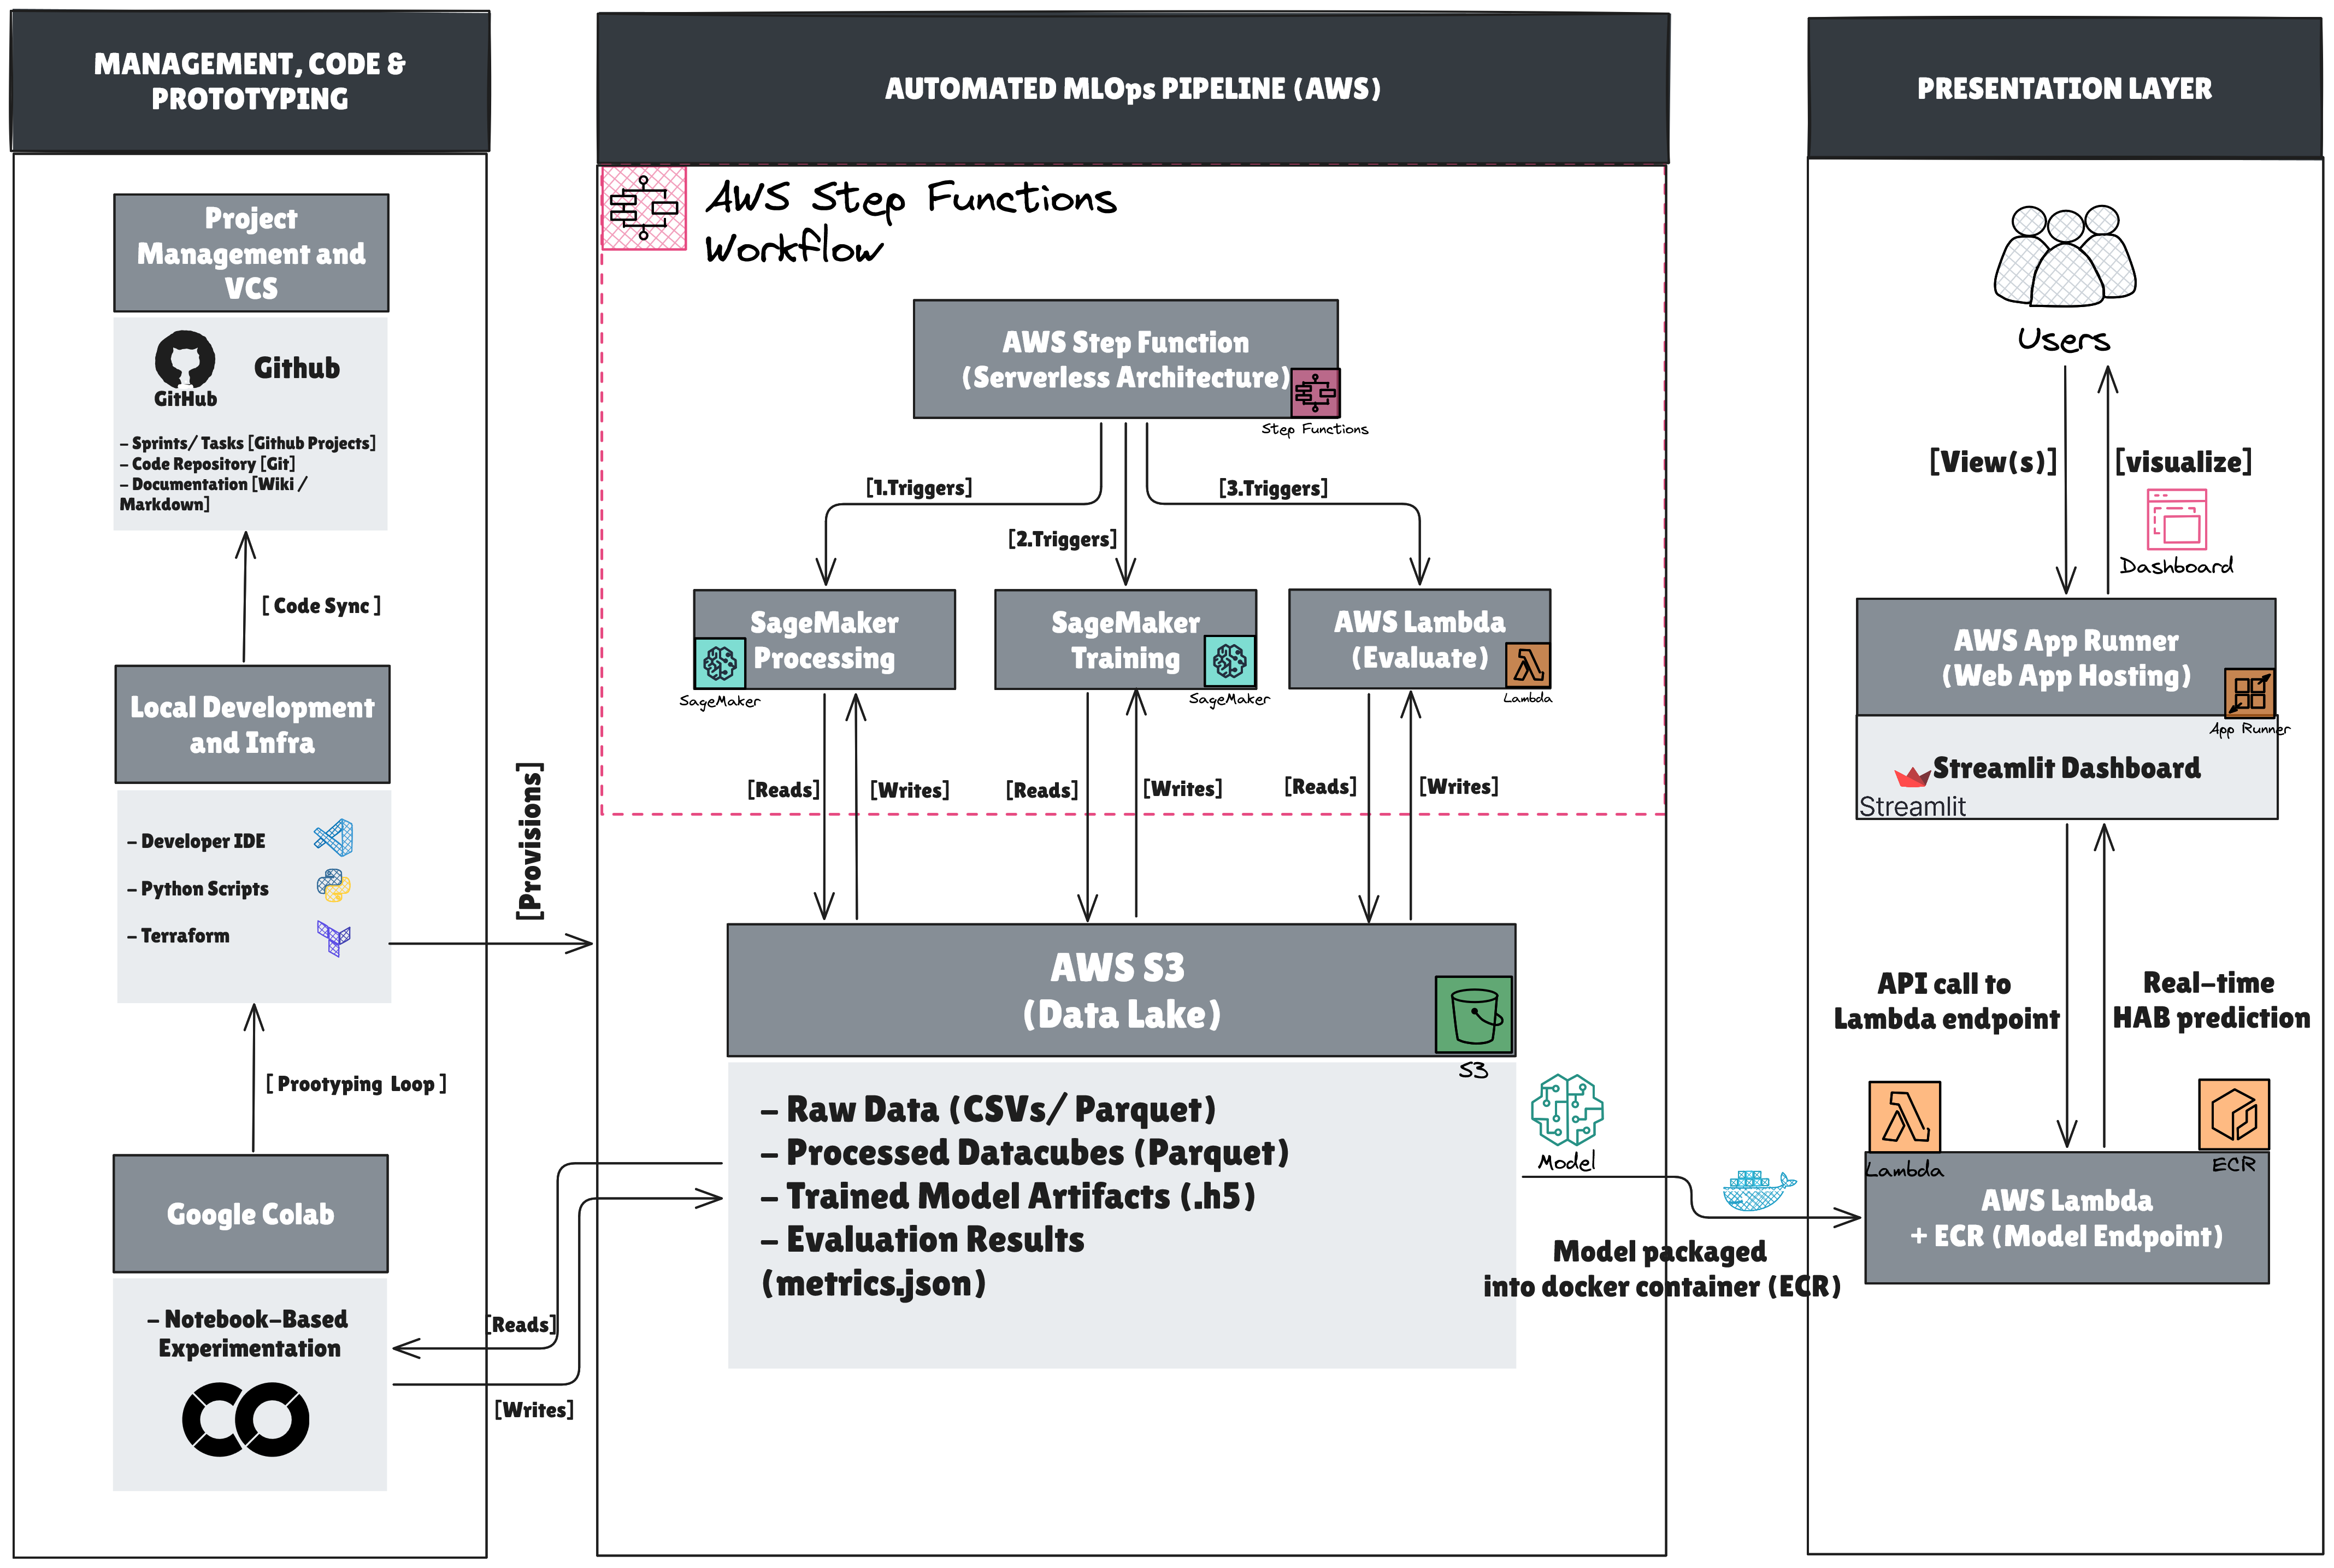
\includegraphics[width=\linewidth]{Project_Architecture.png}
  \caption{System architecture for HAB detection and prediction. The pipeline integrates local development, version control, and notebook experimentation with an automated AWS-based MLOps workflow using Step Functions, SageMaker, and Lambda. Outputs are stored in S3 and served through a Streamlit dashboard hosted on AWS App Runner for real-time HAB prediction.}
  \label{fig:hab-architecture}
\end{figure}


%%------------------------------------------------
\section{Data Plan}
%%------------------------------------------------



%%------------------------------------------------
\section{GitHub Repository}
%%------------------------------------------------


%%------------------------------------------------
\section{Team Management}
%%------------------------------------------------
The team follows a sprint-based approach using GitHub Projects to track progress and assign tasks. Weekly sync-up meetings are held to review milestones, address blockers, and redistribute work as needed.

We maintain a shared GitHub repository where all members regularly commit updates to ensure version control and collaboration. Communication is done through a dedicated group chat and short catch-up calls when necessary.

Everyone is accountable for their role, but we also coordinate cross-functionally to ensure smooth integration of all components.


%%------------------------------------------------
% End 
%%------------------------------------------------


\bibliographystyle{plain}
\bibliography{references} 

\end{document}